\documentclass{standalone}

\usepackage{tikz}

\usetikzlibrary{positioning, chains, shapes.geometric, fit, shapes, arrows.meta, calc}

\begin{document}

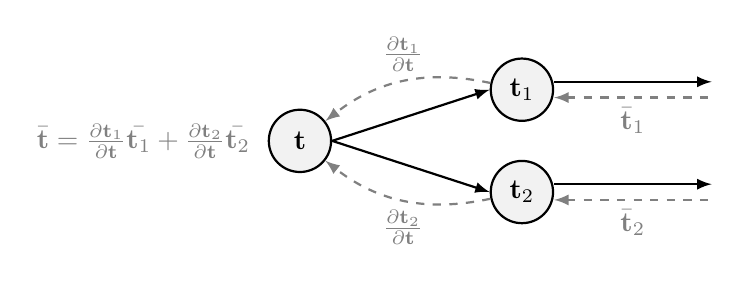
\begin{tikzpicture}[
    >=LaTeX, % Use default LaTeX arrows
    % Styles 
    node/.style={ % Input or output node
        circle,
        minimum width=2.25em,
        draw,
        fill=gray!10,
        thick
    },
    arrow/.style={
        -latex,
        thick
    },
    backprop/.style={ % Backpropagation arrows
        arrow,
        dashed,
        gray
    }
]
    % Computational graph nodes
    \node[node] (t) {$\mathbf{t}$};
    \node[node] (t1) [right=of t, xshift=1cm, yshift=0.65cm] {$\mathbf{t}_1$};
    \node[node] (t2) [right=of t, xshift=1cm, yshift=-0.65cm] {$\mathbf{t}_2$};
    \node[gray] (tlabel) [left=0.1cm of t] {$\bar{\mathbf{t}} = 
    \frac{\partial \mathbf{t}_1}{\partial \mathbf{t}}\bar{\mathbf{t}_1} + \frac{\partial \mathbf{t}_2}{\partial \mathbf{t}}\bar{\mathbf{t}_2}$};

    % Computational graph edges
    \draw[arrow] (t.east) -- (t1.west);
    \draw[arrow] (t.east) -- (t2.west);
    \draw[arrow] (t1.east) +(0cm,0.1cm) -- +(2cm,0.1cm) node[midway, above] {};
    \draw[arrow] (t2.east) +(0cm,0.1cm) -- +(2cm,0.1cm) node[midway, above] {};

    % Backpropagation arrows with partial derivatives
    \draw[backprop, bend right=25] (t1) to node[midway, above] {$\frac{\partial \mathbf{t}_1}{\partial \mathbf{t}}$} (t);
    \draw[backprop, bend left=25] (t2) to node[midway, below] {$\frac{\partial \mathbf{t}_2}{\partial \mathbf{t}}$} (t);
    \draw[backprop, latex-] (t1.east) +(0cm,-0.1cm) -- +(2cm,-0.1cm) node[midway, below] {$\bar{\mathbf{t}}_1$};
    \draw[backprop, latex-] (t2.east) +(0cm,-0.1cm) -- +(2cm,-0.1cm) node[midway, below] {$\bar{\mathbf{t}}_2$};
\end{tikzpicture}

\end{document}